% docs/projektbeschreibung.tex -- Interferosim project description
% Version 1.0.2 (2026-10-11) -- removed "e.g. a VU" from target audience
% Version 1.0.1 (2026-10-11) -- added OH maser lines to sky models
% Version 1.0.0 (2026-10-11)
% Compile with: pdflatex projektbeschreibung.tex
\documentclass[11pt,a4paper]{article}

\usepackage[utf8]{inputenc}
\usepackage[T1]{fontenc}
\usepackage[english]{babel}
\usepackage{lmodern}
\usepackage[margin=2.5cm]{geometry}
\usepackage{booktabs}
\usepackage{tabularx}
\usepackage{enumitem}
\usepackage{xcolor}
\usepackage{tikz}
\usepackage[hidelinks]{hyperref}

\definecolor{phase}{RGB}{40,90,160}
\definecolor{buffer}{RGB}{170,170,170}

\title{\textbf{Interferosim}\\[0.3em]
\large An open-source simulator for radio interferometry\\
Project description}
\author{DI Erich Schubert}
\date{Version 1.0.2 -- 11 October 2026}

\begin{document}
\maketitle

% ------------------------------------------------------------------
\section{Scope of the software}

Interferosim is an open-source Python package for simulating radio
interferometers, from a simple two-element system up to small arrays.
It comes with a set of interactive Jupyter notebooks in which sliders
and dropdowns (ipywidgets) control the array layout, the sky model and
the observing parameters. Plots update directly in the notebook, and
code and explanatory text sit side by side, so the notebooks also serve
as course material.

The software covers the full processing chain:

\begin{itemize}[noitemsep]
  \item \textbf{Sky models:} point sources, extended emission,
        HI 21\,cm maps (1420.406\,MHz) and OH maser sources
        (18\,cm band). The OH ground-state transitions are
        1612.231\,MHz (satellite line), 1665.402\,MHz and
        1667.359\,MHz (main lines) and 1720.530\,MHz (satellite line).
        % v1.0.1: OH maser lines added alongside HI
  \item \textbf{Instrument:} antenna positions, baselines, observing
        frequency and duration.
  \item \textbf{Observation:} uv-coverage including Earth rotation
        synthesis, visibility calculation, optional noise.
  \item \textbf{Imaging:} dirty image and dirty beam (PSF).
  \item \textbf{Deconvolution:} Högbom-CLEAN and Wiener filter, with
        metrics for a direct comparison of the results.
  \item \textbf{Visualisation:} array layout, uv-plane, fringes, PSF
        and reconstructed image for every step.
\end{itemize}

The goal is to make visible how choices on the instrument side affect
the final image.

% ------------------------------------------------------------------
\section{Target audience}

\begin{itemize}
  \item \textbf{Students} in astronomy and physics courses
        who want a hands-on way into aperture synthesis instead of only
        reading the formulas.
  \item \textbf{Lecturers} who need ready-to-use demonstrations and
        exercises.
  \item \textbf{Amateur radio astronomers} planning their own
        interferometer, who can test baseline lengths, antenna placement
        and expected resolution before building any hardware.
\end{itemize}

No deep programming knowledge is needed to use the notebooks. The
modular core package stays open for extensions. If the notebooks run on
JupyterHub or Binder, students do not need to install anything.

% ------------------------------------------------------------------
\section{Development plan}

Start: Monday, 12 October 2026.

\medskip
\noindent
\small
\begin{tabularx}{\textwidth}{@{}>{\raggedright\arraybackslash}p{3.6cm}
  >{\raggedright\arraybackslash}X l r@{}}
\toprule
\textbf{Phase} & \textbf{Content} & \textbf{Period} & \textbf{Weeks}\\
\midrule
1. Concept \& architecture & Requirements, package structure, data
  formats, repository, licence & 12.10.--25.10.2026 & 2\\
2. Core simulation & Sky models, array geometry, uv-coverage,
  visibility calculation & 26.10.--22.11.2026 & 4\\
3. Imaging \& deconvolution & Dirty image/beam, Högbom-CLEAN, Wiener
  filter, comparison metrics & 23.11.--20.12.2026 & 4\\
\textit{Christmas break / buffer} & & 21.12.2026--03.01.2027 & 2\\
4. Interactive notebooks & ipywidgets controls, interactive plots, one
  notebook per topic (basics, uv-coverage, imaging, deconvolution)
  & 04.01.--24.01.2027 & 3\\
5. Testing \& validation & Unit tests for the core package, automated
  notebook runs (e.g.\ nbval) & 25.01.--07.02.2027 & 2\\
6. Documentation \& teaching material & Exercises in the notebooks,
  LaTeX handout, release v1.0.0 & 08.02.--21.02.2027 & 2\\
\midrule
\textbf{Total} & 17 weeks of work + 2 weeks buffer
  & 12.10.2026--21.02.2027 & \textbf{19}\\
\bottomrule
\end{tabularx}
\normalsize

\bigskip
% Gantt-style overview: x unit = 1 week, week 0 = 12.10.2026
\begin{center}
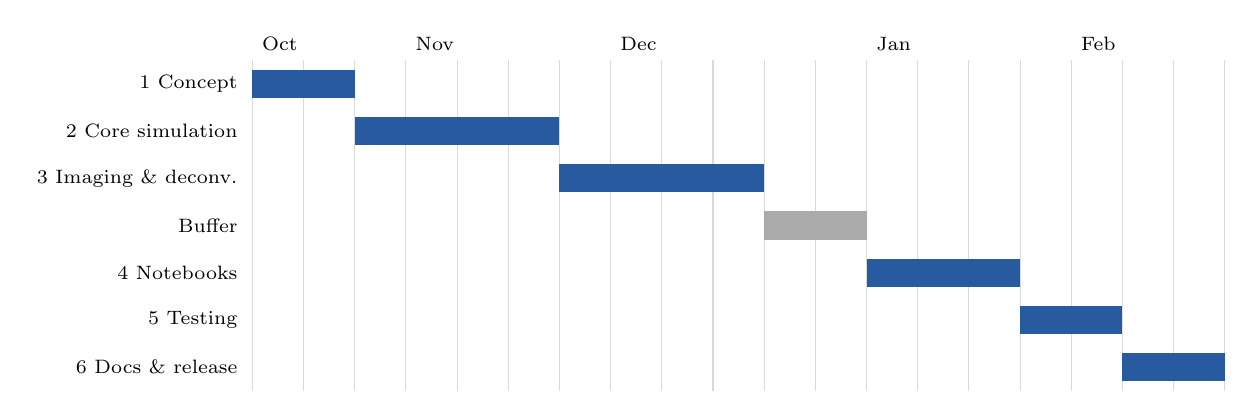
\begin{tikzpicture}[x=0.65cm,y=0.6cm]
  % week grid
  \foreach \w in {0,...,19}
    \draw[gray!30] (\w,0.5) -- (\w,-6.5);
  % month labels (approximate week offsets)
  \foreach \w/\m in {0/Oct,3/Nov,7/Dec,12/Jan,16/Feb}
    \node[anchor=south west,font=\scriptsize] at (\w,0.5) {\m};
  % phases: start week / length / label / row
  \foreach \s/\l/\t/\r/\c in {
      0/2/{1 Concept}/0/phase,
      2/4/{2 Core simulation}/1/phase,
      6/4/{3 Imaging \& deconv.}/2/phase,
      10/2/{Buffer}/3/buffer,
      12/3/{4 Notebooks}/4/phase,
      15/2/{5 Testing}/5/phase,
      17/2/{6 Docs \& release}/6/phase}{
    \fill[\c] (\s,-\r+0.3) rectangle ++(\l,-0.6);
    \node[anchor=east,font=\scriptsize] at (-0.1,-\r) {\t};
  }
\end{tikzpicture}
\end{center}

\noindent
The core package is independent of the user interface. A PySide6
desktop front end can therefore be added later on top of the same code
without changing the simulation or imaging modules.

\end{document}
